\documentclass[11pt]{article}
\usepackage[utf8]{inputenc}
\usepackage{graphicx}
\usepackage{caption}
\usepackage{subcaption}
\usepackage{amsmath}
\usepackage{float}


\title{
	{Computer Vision 2 - Assignment 1\\
	 Iterative Closest Point - ICP}
}
\author{
Selene Baez Santamaria (10985417) - Ildefonso Ferreira ()}
\date{\today}

\begin{document}

\maketitle

\section{ICP}
In this assignment we create a function called \textit{own\_ICP} which implements the Iterative Closest Point algorithm. This function takes as arguments a base point cloud and a target point cloud, and a parameter \textit{k} for the number of points to be sampled. 

\subsection{Implementation}

\begin{enumerate}
	\item \textit{Phase 1:} In this phase we find the corresponding points. To do so we use the function provided by the assignment package \textit{dist2} to find the distance among two sets of points. For each point in the base cloud we match it with the point in the target cloud that returns the lowest distance. 
	
	Our first approach was to use brute force and compare all points in one cloud to points in the second cloud. However, this lead to problems regarding memory capacity. Thus, we chose to sample the points to be matched to work within such limitations.
	
	A second approach led us to sample the first \textit{k} elements in each cloud and compare them.
	
	An ideal approach is to get the most significant points from the clouds and compare them. %TODO try to implement this
	
	\item \textit{Phase 2:} Secondly, we find the geometric centers of each cloud and translate the points to center them. 
	
	\item \textit{Phase 3:} Next, we apply single value decomposition using Matlab's built in function \textit{svd}. The matrix to be decomposed is $A$, the covariance matrix between both clouds. 
	
	\item \textit{Phase 4:} We proceed to calculate the Rotation and translation matrices
	
	\item \textit{Phase 5:} Finally we calculate the average distances between the base and the transformed clouds. 
	
	We implemented two smart stopping conditions: the first stops if the distance is already within a certain threshold. The selected threshold is $ threshold = 0.001 $. The second condition limits the number of iterations to 30, since literature shows that this is often where the rate of significant improvement slows down.
\end{enumerate}

We tested our implementation with the given \textit{source.mat} and \textit{target.mat} files. Figure \ref{fig:test} we present a visualization of the results obtained with these point clouds 

\begin{figure}[h]
	\centering
	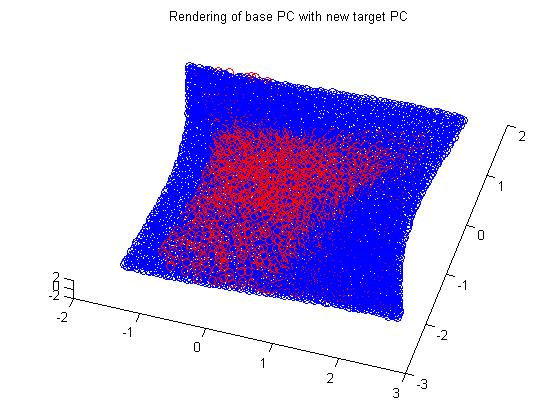
\includegraphics[width=1\textwidth]{img/test_clouds.jpg}
	\caption{Alignment of source and target point clouds provided. Blue points correspond to source cloud and red points correspond to target cloud}
	\label{fig:test}
\end{figure}

\section{Merging scenes}


\subsection{Estimating camera poses using consecutive frames}



\subsection{Estimating camera poses using iterative merging}



\section{Reflection}

\subsection{Drawbacks of ICP}
The performance heavily depends on the initial orientation of the point clouds. 

\subsection{Improvements}
Selection of significant points.



\end{document}

